\documentclass[twoside]{book}

% Packages required by doxygen
\usepackage{fixltx2e}
\usepackage{calc}
\usepackage{doxygen}
\usepackage[export]{adjustbox} % also loads graphicx
\usepackage{graphicx}
\usepackage[utf8]{inputenc}
\usepackage{makeidx}
\usepackage{multicol}
\usepackage{multirow}
\PassOptionsToPackage{warn}{textcomp}
\usepackage{textcomp}
\usepackage[nointegrals]{wasysym}
\usepackage[table]{xcolor}

% Font selection
\usepackage[T1]{fontenc}
\usepackage[scaled=.90]{helvet}
\usepackage{courier}
\usepackage{amssymb}
\usepackage{sectsty}
\renewcommand{\familydefault}{\sfdefault}
\allsectionsfont{%
  \fontseries{bc}\selectfont%
  \color{darkgray}%
}
\renewcommand{\DoxyLabelFont}{%
  \fontseries{bc}\selectfont%
  \color{darkgray}%
}
\newcommand{\+}{\discretionary{\mbox{\scriptsize$\hookleftarrow$}}{}{}}

% Page & text layout
\usepackage{geometry}
\geometry{%
  a4paper,%
  top=2.5cm,%
  bottom=2.5cm,%
  left=2.5cm,%
  right=2.5cm%
}
\tolerance=750
\hfuzz=15pt
\hbadness=750
\setlength{\emergencystretch}{15pt}
\setlength{\parindent}{0cm}
\setlength{\parskip}{3ex plus 2ex minus 2ex}
\makeatletter
\renewcommand{\paragraph}{%
  \@startsection{paragraph}{4}{0ex}{-1.0ex}{1.0ex}{%
    \normalfont\normalsize\bfseries\SS@parafont%
  }%
}
\renewcommand{\subparagraph}{%
  \@startsection{subparagraph}{5}{0ex}{-1.0ex}{1.0ex}{%
    \normalfont\normalsize\bfseries\SS@subparafont%
  }%
}
\makeatother

% Headers & footers
\usepackage{fancyhdr}
\pagestyle{fancyplain}
\fancyhead[LE]{\fancyplain{}{\bfseries\thepage}}
\fancyhead[CE]{\fancyplain{}{}}
\fancyhead[RE]{\fancyplain{}{\bfseries\leftmark}}
\fancyhead[LO]{\fancyplain{}{\bfseries\rightmark}}
\fancyhead[CO]{\fancyplain{}{}}
\fancyhead[RO]{\fancyplain{}{\bfseries\thepage}}
\fancyfoot[LE]{\fancyplain{}{}}
\fancyfoot[CE]{\fancyplain{}{}}
\fancyfoot[RE]{\fancyplain{}{\bfseries\scriptsize Generated by Doxygen }}
\fancyfoot[LO]{\fancyplain{}{\bfseries\scriptsize Generated by Doxygen }}
\fancyfoot[CO]{\fancyplain{}{}}
\fancyfoot[RO]{\fancyplain{}{}}
\renewcommand{\footrulewidth}{0.4pt}
\renewcommand{\chaptermark}[1]{%
  \markboth{#1}{}%
}
\renewcommand{\sectionmark}[1]{%
  \markright{\thesection\ #1}%
}

% Indices & bibliography
\usepackage{natbib}
\usepackage[titles]{tocloft}
\setcounter{tocdepth}{3}
\setcounter{secnumdepth}{5}
\makeindex

% Hyperlinks (required, but should be loaded last)
\usepackage{ifpdf}
\ifpdf
  \usepackage[pdftex,pagebackref=true]{hyperref}
\else
  \usepackage[ps2pdf,pagebackref=true]{hyperref}
\fi
\hypersetup{%
  colorlinks=true,%
  linkcolor=blue,%
  citecolor=blue,%
  unicode%
}

% Custom commands
\newcommand{\clearemptydoublepage}{%
  \newpage{\pagestyle{empty}\cleardoublepage}%
}

\usepackage{caption}
\captionsetup{labelsep=space,justification=centering,font={bf},singlelinecheck=off,skip=4pt,position=top}

%===== C O N T E N T S =====

\begin{document}

% Titlepage & ToC
\hypersetup{pageanchor=false,
             bookmarksnumbered=true,
             pdfencoding=unicode
            }
\pagenumbering{alph}
\begin{titlepage}
\vspace*{7cm}
\begin{center}%
{\Large My Project }\\
\vspace*{1cm}
{\large Generated by Doxygen 1.8.13}\\
\end{center}
\end{titlepage}
\clearemptydoublepage
\pagenumbering{roman}
\tableofcontents
\clearemptydoublepage
\pagenumbering{arabic}
\hypersetup{pageanchor=true}

%--- Begin generated contents ---
\chapter{File Index}
\section{File List}
Here is a list of all documented files with brief descriptions\+:\begin{DoxyCompactList}
\item\contentsline{section}{{\bfseries game.\+h} }{\pageref{game_8h}}{}
\item\contentsline{section}{\hyperlink{haut__bas_8c}{haut\+\_\+bas.\+c} }{\pageref{haut__bas_8c}}{}
\item\contentsline{section}{\hyperlink{main_8c}{main.\+c} \\*Testing Program }{\pageref{main_8c}}{}
\end{DoxyCompactList}

\chapter{File Documentation}
\hypertarget{fonct_8c}{}\section{fonct.\+c File Reference}
\label{fonct_8c}\index{fonct.\+c@{fonct.\+c}}
{\ttfamily \#include \char`\"{}S\+D\+L/\+S\+D\+L.\+h\char`\"{}}\newline
{\ttfamily \#include $<$stdio.\+h$>$}\newline
{\ttfamily \#include $<$stdlib.\+h$>$}\newline
{\ttfamily \#include $<$S\+D\+L/\+S\+D\+L\+\_\+mixer.\+h$>$}\newline
{\ttfamily \#include $<$S\+D\+L/\+S\+D\+L\+\_\+image.\+h$>$}\newline
{\ttfamily \#include $<$S\+D\+L/\+S\+D\+L\+\_\+ttf.\+h$>$}\newline
{\ttfamily \#include \char`\"{}fonct.\+h\char`\"{}}\newline
Include dependency graph for fonct.\+c\+:
\nopagebreak
\begin{figure}[H]
\begin{center}
\leavevmode
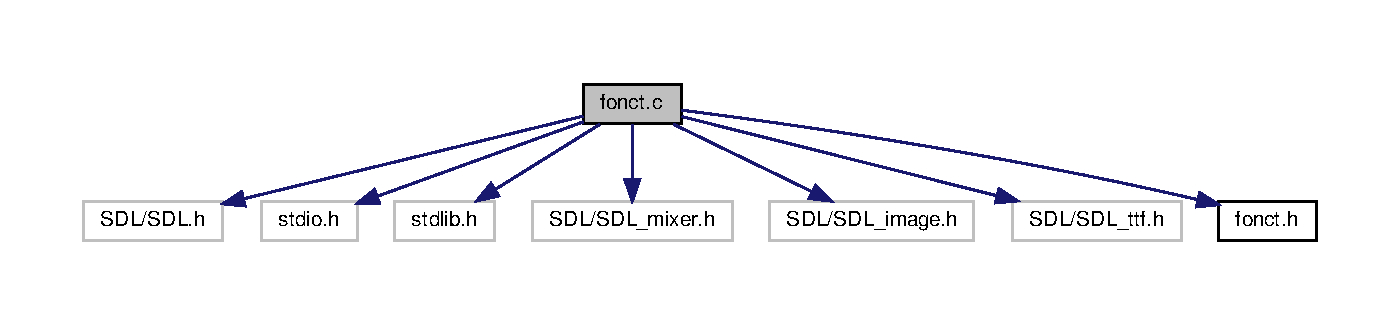
\includegraphics[width=350pt]{fonct_8c__incl}
\end{center}
\end{figure}
\subsection*{Functions}
\begin{DoxyCompactItemize}
\item 
S\+D\+L\+\_\+\+Rect \hyperlink{fonct_8c_ae39ebd4832e965d2e3a5cf2d5b85705b}{map\+\_\+initial} ()
\begin{DoxyCompactList}\small\item\em To initialize the map b . \end{DoxyCompactList}\end{DoxyCompactItemize}


\subsection{Function Documentation}
\mbox{\Hypertarget{fonct_8c_ae39ebd4832e965d2e3a5cf2d5b85705b}\label{fonct_8c_ae39ebd4832e965d2e3a5cf2d5b85705b}} 
\index{fonct.\+c@{fonct.\+c}!map\+\_\+initial@{map\+\_\+initial}}
\index{map\+\_\+initial@{map\+\_\+initial}!fonct.\+c@{fonct.\+c}}
\subsubsection{\texorpdfstring{map\+\_\+initial()}{map\_initial()}}
{\footnotesize\ttfamily S\+D\+L\+\_\+\+Rect map\+\_\+initial (\begin{DoxyParamCaption}\item[{void}]{ }\end{DoxyParamCaption})}



To initialize the map b . 


\begin{DoxyParams}{Parameters}
{\em b} & the map \\
\hline
{\em url} & the url of the image \\
\hline
\end{DoxyParams}
\begin{DoxyReturn}{Returns}
Nothing 
\end{DoxyReturn}
Here is the caller graph for this function\+:
\nopagebreak
\begin{figure}[H]
\begin{center}
\leavevmode
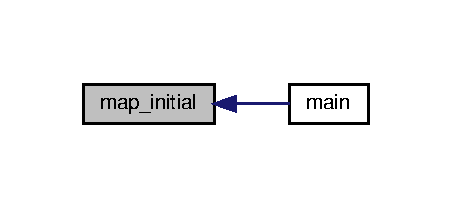
\includegraphics[width=217pt]{fonct_8c_ae39ebd4832e965d2e3a5cf2d5b85705b_icgraph}
\end{center}
\end{figure}

\hypertarget{fonct_8h}{}\section{fonct.\+h File Reference}
\label{fonct_8h}\index{fonct.\+h@{fonct.\+h}}
This graph shows which files directly or indirectly include this file\+:
\nopagebreak
\begin{figure}[H]
\begin{center}
\leavevmode
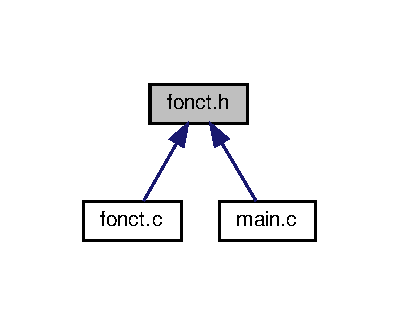
\includegraphics[width=192pt]{fonct_8h__dep__incl}
\end{center}
\end{figure}
\subsection*{Functions}
\begin{DoxyCompactItemize}
\item 
S\+D\+L\+\_\+\+Rect \hyperlink{fonct_8h_a8e4d9e8971ccad2852b2a27b1b49ab67}{map\+\_\+initial} (void)
\begin{DoxyCompactList}\small\item\em To initialize the map b . \end{DoxyCompactList}\item 
void \hyperlink{fonct_8h_ac1811c26ff037cd03a27f99a5a8d01ac}{map\+\_\+2} (S\+D\+L\+\_\+\+Rect positionecran3)
\end{DoxyCompactItemize}


\subsection{Function Documentation}
\mbox{\Hypertarget{fonct_8h_ac1811c26ff037cd03a27f99a5a8d01ac}\label{fonct_8h_ac1811c26ff037cd03a27f99a5a8d01ac}} 
\index{fonct.\+h@{fonct.\+h}!map\+\_\+2@{map\+\_\+2}}
\index{map\+\_\+2@{map\+\_\+2}!fonct.\+h@{fonct.\+h}}
\subsubsection{\texorpdfstring{map\+\_\+2()}{map\_2()}}
{\footnotesize\ttfamily void map\+\_\+2 (\begin{DoxyParamCaption}\item[{S\+D\+L\+\_\+\+Rect}]{positionecran3 }\end{DoxyParamCaption})}

\mbox{\Hypertarget{fonct_8h_a8e4d9e8971ccad2852b2a27b1b49ab67}\label{fonct_8h_a8e4d9e8971ccad2852b2a27b1b49ab67}} 
\index{fonct.\+h@{fonct.\+h}!map\+\_\+initial@{map\+\_\+initial}}
\index{map\+\_\+initial@{map\+\_\+initial}!fonct.\+h@{fonct.\+h}}
\subsubsection{\texorpdfstring{map\+\_\+initial()}{map\_initial()}}
{\footnotesize\ttfamily S\+D\+L\+\_\+\+Rect map\+\_\+initial (\begin{DoxyParamCaption}\item[{void}]{ }\end{DoxyParamCaption})}



To initialize the map b . 


\begin{DoxyParams}{Parameters}
{\em b} & the map \\
\hline
{\em url} & the url of the image \\
\hline
\end{DoxyParams}
\begin{DoxyReturn}{Returns}
Nothing 
\end{DoxyReturn}
Here is the caller graph for this function\+:
\nopagebreak
\begin{figure}[H]
\begin{center}
\leavevmode
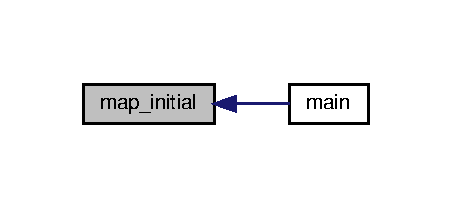
\includegraphics[width=217pt]{fonct_8h_a8e4d9e8971ccad2852b2a27b1b49ab67_icgraph}
\end{center}
\end{figure}

\hypertarget{main_8c}{}\section{main.\+c File Reference}
\label{main_8c}\index{main.\+c@{main.\+c}}
{\ttfamily \#include $<$stdlib.\+h$>$}\\*
{\ttfamily \#include $<$stdio.\+h$>$}\\*
{\ttfamily \#include $<$S\+D\+L/\+S\+D\+L.\+h$>$}\\*
{\ttfamily \#include $<$S\+D\+L/\+S\+D\+L\+\_\+image.\+h$>$}\\*
{\ttfamily \#include \char`\"{}background.\+h\char`\"{}}\\*
Include dependency graph for main.\+c\+:\nopagebreak
\begin{figure}[H]
\begin{center}
\leavevmode
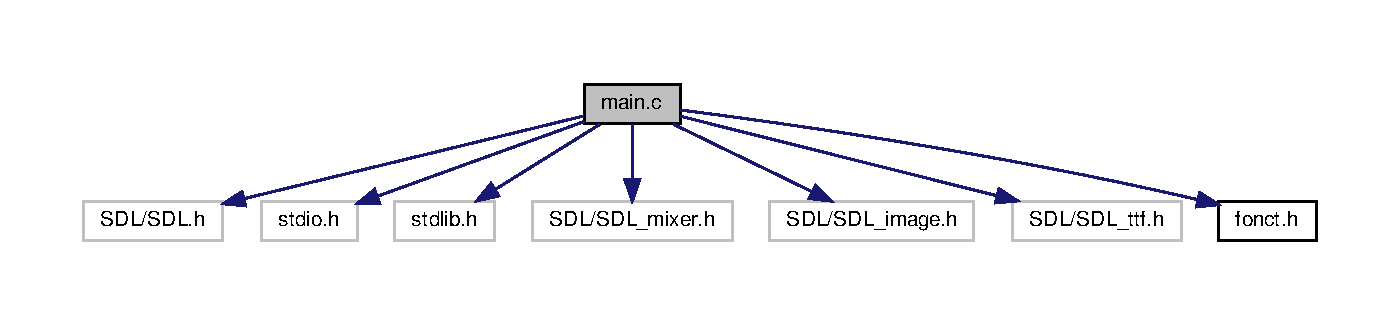
\includegraphics[width=350pt]{main_8c__incl}
\end{center}
\end{figure}
\subsection*{Functions}
\begin{DoxyCompactItemize}
\item 
int {\bfseries main} (int argc, char $\ast$argv\mbox{[}$\,$\mbox{]})\hypertarget{main_8c_a0ddf1224851353fc92bfbff6f499fa97}{}\label{main_8c_a0ddf1224851353fc92bfbff6f499fa97}

\end{DoxyCompactItemize}


\subsection{Detailed Description}
\begin{DoxyAuthor}{Author}
wael 
\end{DoxyAuthor}
\begin{DoxyDate}{Date}
Mai 14, 2020 
\end{DoxyDate}

%--- End generated contents ---

% Index
\backmatter
\newpage
\phantomsection
\clearemptydoublepage
\addcontentsline{toc}{chapter}{Index}
\printindex

\end{document}
